\chapter{Architecture et implémentation}
\label{chapitre:architecture}

Ce chapitre décrit la réalisation logicielle du système, c'est-à-dire la traduction des choix
méthodologiques du chapitre précédent en un programme concret. Il présente d'abord
l'architecture en couches et les principes de conception qui la structurent, puis les choix
d'implémentation, la stratégie de tests et le détail des algorithmes de détection retenus
(Isolation Forest et Local Outlier Factor). Il aborde ensuite les technologies employées,
l'interface interactive de visualisation, ainsi que les mécanismes de traçabilité et de
reproductibilité. L'objectif est de rendre explicite la manière dont la méthodologie se
concrétise en un système modulaire, interprétable et auditable.

% =====================================================================
\section{Architecture logicielle}
% =====================================================================

L'architecture logicielle est volontairement découpée en couches fonctionnelles, séparant la
logique métier, la présentation, la validation expérimentale et la traçabilité. La séparation
des responsabilités limite le couplage entre prétraitement, modélisation et évaluation, source
de dette technique dans les systèmes d'apprentissage automatique \citep{sculley2015hidden}. Le
système s'organise autour de cinq composantes fonctionnelles. Le Tableau~\ref{tab:modules} en
précise le rôle et le contrat d'entrée-sortie, tandis que la Figure~\ref{fig:architecture_modules}
en montre l'organisation en couches et les dépendances. Les flèches pleines y indiquent un appel
direct entre le cœur algorithmique et les couches externes, les pointillées une dépendance de
configuration.

\begin{table}[H]
    \centering
    \small
    \caption{Composantes fonctionnelles du système de détection.}
    \label{tab:modules}
    \begin{tabular}{>{\raggedright\arraybackslash}p{3.0cm}
                    >{\raggedright\arraybackslash}p{6.3cm}
                    >{\raggedright\arraybackslash}p{3.8cm}}
        \toprule
        \textbf{Composante} & \textbf{Rôle} & \textbf{Entrée / Sortie} \\
        \midrule
        Chargement et filtrage & Normalisation des formats, couverture capteur & CSV $\rightarrow$ série nettoyée \\
        Extraction de \textit{features} & Z-scores robustes, \textit{features}, moyennes mobiles & Série $\rightarrow$ matrice de \textit{features} \\
        Détection d'anomalies & Isolation Forest par vache, scores et flags & Features $\rightarrow$ anomalies \\
        Règles métier & Persistance, cohérence multi-signaux, cooldown & Anomalies $\rightarrow$ épisodes \\
        Orchestration & Chaînage bout en bout des quatre étapes & CSV brut $\rightarrow$ notifications \\
        \bottomrule
    \end{tabular}
\end{table}

\begin{figure}[H]
    \centering
    \resizebox{\textwidth}{!}{%
    \begin{tikzpicture}[
        module/.style={rectangle, draw=black!70, rounded corners=3pt, minimum height=0.9cm,
                       minimum width=2.4cm, align=center, font=\small, inner sep=12pt},
        group/.style={rectangle, draw=black!50, dashed, rounded corners=5pt, inner sep=8pt},
        arrow/.style={-{Stealth[length=2.5mm]}, thick, black!80},
        darrow/.style={-{Stealth[length=2.5mm]}, thick, dashed, black!40},
    ]
        % Core modules
        \node[module, fill=gray!12] (io) {Chargement\\[-7pt]et filtrage};
        \node[module, fill=ifblue!15, right=1.2cm of io] (feat) {Extraction\\[-7pt]de \textit{features}};
        \node[module, fill=loforange!12, right=1.2cm of feat] (model) {Détection\\[-7pt](IF)};
        \node[module, fill=rulegreen!15, right=1.2cm of model] (alerts) {Règles\\[-7pt]métier};

        \path (feat) -- (model) coordinate[midway] (fm);
        \node[module, fill=gray!8, below=1cm of fm] (config) {Configuration\\[-7pt]centralisée};
        \node[module, fill=gray!8, above=1cm of fm] (pipeline) {Orchestration};

        % Group
        \node[group, fit=(io)(feat)(model)(alerts)(config)(pipeline),
              label={[font=\small\bfseries, black]above left:Coeur algorithmique}] (corebox) {};

        % External
        \node[module, fill=purple!8, right=1.5cm of alerts] (ui) {Interface\\[-7pt]interactive};
        \node[module, fill=yellow!10, below=1cm of ui] (scripts) {Validation\\[-7pt]expérimentale};

        % Arrows - flux principal (horizontales)
        \draw[arrow] (io) -- (feat);
        \draw[arrow] (feat) -- (model);
        \draw[arrow] (model) -- (alerts);

        % Arrows - orchestration (verticales vers le bas)
        \draw[arrow] (pipeline.west) -- ++(0,0) -| (io.north);
        \draw[arrow] (pipeline.east) -- ++(0,0) -| (alerts.north);

        % Arrows - configuration (verticales vers le haut, s'arretent au bord)
        \draw[darrow] (config.west) -- ++(0,0) -| (io.south);
        \draw[darrow] (config) -- (feat.south);
        \draw[darrow] (config) -- (model.south);
        \draw[darrow] (config.east) -- ++(0,0) -| (alerts.south);

        % Arrows - vers externe
        \draw[arrow] (corebox.east |- ui) -- (ui);
        \draw[darrow] (corebox.east |- scripts) -- (scripts);
    \end{tikzpicture}%
    }
    \caption{Diagramme de dépendances entre les composantes du pipeline.}
    \label{fig:architecture_modules}
\end{figure}

En pratique, le découpage en couches fonctionnelles permet à l'interface, à la validation
expérimentale et au coeur de détection d'évoluer indépendamment. L'interface expose le pipeline et ses
sorties de manière visuelle, tandis que la logique de détection reste concentrée dans les
composantes du coeur algorithmique.

L'architecture du système repose sur quatre principes de conception logicielle, résumés
dans le Tableau~\ref{tab:principes_conception}. Ces principes ne sont pas des choix
esthétiques; ils répondent à des contraintes concrètes rencontrées lors du développement
et de la validation du pipeline.

\begin{table}[H]
    \centering
    \caption{Principes de conception logicielle appliqués au pipeline de détection
    et leur justification pratique.}
    \label{tab:principes_conception}
    \begin{tabular}{>{\raggedright\arraybackslash}p{3cm}
                    >{\raggedright\arraybackslash}p{4.5cm}
                    >{\raggedright\arraybackslash}p{5cm}}
        \toprule
        \textbf{Principe} & \textbf{Mise en oeuvre} & \textbf{Bénéfice observé} \\
        \midrule
        Séparation des responsabilités
        & Une composante par étape du pipeline
        & Test en isolation, localisation rapide des bugs \\
        \addlinespace
        Configuration centralisée
        & Paramètres dans un module unique, gelé après validation
        & Aucune incohérence entre validation et interface \\
        \addlinespace
        Immutabilité des artefacts
        & Résultats de référence vérifiés par SHA-256
        & Altérations détectées avant publication \\
        \addlinespace
        Reproductibilité par seeds
        & Seeds aléatoires fixés et documentés
        & Reproductibilité bit à bit (mêmes dépendances) \\
        \bottomrule
    \end{tabular}
\end{table}

Le premier principe, la séparation des responsabilités, confine chaque étape du pipeline à une
composante unique, condition d'un test isolé et d'un diagnostic rapide des anomalies. La
configuration centralisée regroupe ensuite tous les paramètres dans un module unique gelé après
validation, ce qui élimine tout écart entre la validation robuste et l'interface. L'immutabilité
des artefacts de référence, contrôlée par empreintes SHA-256, rend visible toute altération
accidentelle avant publication. La reproductibilité, enfin, repose sur le gel et la documentation
des seeds aléatoires, garantissant des résultats identiques bit à bit à environnement de
dépendances constant.

L'ensemble de ces principes a été appliqué dès le début du développement, ce qui a permis de conduire
les 9\,504~exécutions expérimentales des validations robustes. En
pratique, la discipline de tests de non-régression a permis de détecter deux incidents de
modification involontaire de résultats lors de refactorings, avant qu'ils n'affectent les
conclusions.

\FloatBarrier
% =====================================================================
\section{Choix d'implémentation}
% =====================================================================

Plusieurs décisions d'implémentation visent explicitement la maintenabilité et la
reproductibilité. Ces choix s'inscrivent dans les bonnes pratiques identifiées par la
littérature en systèmes d'apprentissage automatique appliqués, où la reproductibilité est souvent le premier
facteur de crédibilité \citep{sculley2015hidden}. Les sous-sections suivantes détaillent tour à
tour l'organisation du code en façades, la centralisation des paramètres, la séparation entre
logique et présentation et la traçabilité du flux de données.

\subsection{Façades publiques et composantes internes}
L'usage de façades publiques compactes devant des composantes internes plus spécialisées
évite de surcharger l'utilisation du système. Les composantes internes restent modulaires
sans imposer une compréhension détaillée de chaque sous-partie. Par exemple, la composante
d'orchestration expose un point d'entrée unique qui chaîne les quatre étapes sans que
l'appelant ait besoin de connaître les détails de chaque composante.

\subsection{Source unique de vérité pour les paramètres}
Les valeurs du pipeline (seuils de détection, fenêtres de persistance et hyperparamètres du
détecteur) sont centralisées dans une composante de configuration unique, puis gelées après
validation. Ce gel garantit qu'une même configuration sert à la fois la validation robuste et
l'exploitation, ce qui élimine tout risque d'incohérence entre les couches du système. La liste
complète de ces paramètres figés figure au Tableau~\ref{tab:config_finale}
(Chapitre~\ref{chapitre:methodologie}).

\subsection{Séparation logique / présentation}
Les évolutions récentes du système ont principalement porté sur la lisibilité (découpage,
façades, documentation), tandis que l'intégrité des résultats a été protégée par tests
automatisés et vérification d'intégrité. Cette discipline est importante pour un mémoire,
car elle permet d'affirmer qu'une amélioration de structure n'est pas une altération
silencieuse des résultats expérimentaux.

\subsection{Flux de données détaillé}
La Figure~\ref{fig:data_flow} détaille le flux de données à travers les quatre étapes
du pipeline, en précisant les transformations appliquées et les formats intermédiaires.
Chaque étape produit un format intermédiaire documenté, ce qui facilite le débogage et
la reproductibilité des résultats.

\begin{figure}[H]
    \centering
    \resizebox{\textwidth}{!}{%
    \begin{tikzpicture}[
        etape/.style={rectangle, draw=black!60, rounded corners=3pt, minimum height=1cm,
                      minimum width=3cm, align=center, font=\footnotesize, inner sep=10pt},
        donnee/.style={rectangle, draw=black!30, rounded corners=2pt, minimum height=0.7cm,
                       minimum width=2.5cm, align=center, font=\scriptsize, inner sep=5pt,
                       text width=2.8cm, fill=profgray!6},
        arrow/.style={-{Stealth[length=2mm]}, thick, black!60},
    ]
        % Étapes
        \node[etape, fill=gray!12] (s1) at (0,0) {Chargement\\[-7pt]et filtrage};
        \node[etape, fill=ifblue!12] (s2) at (4.2,0) {Extraction\\[-7pt]de \textit{features}};
        \node[etape, fill=loforange!12] (s3) at (8.4,0) {Détection\\[-7pt](IF)};
        \node[etape, fill=rulegreen!12] (s4) at (12.6,0) {Règles\\[-7pt]métier};

        % Sortie finale, placée au-dessus de la dernière étape
        \node[donnee, fill=rulegreen!10] (d4) at (12.6,2) {Épisodes + notifications};

        % Données intermédiaires
        \node[donnee] (d0) at (-3.4,0) {CSV brut (37\,839 lignes)};
        \node[donnee] (d1) at (2.1,-1.8) {Série nettoyée ($\approx$1\,350 bins/vache)};
        \node[donnee] (d2) at (6.3,-1.8) {Matrice \textit{features} ($\approx$50 colonnes)};
        \node[donnee] (d3) at (10.5,-1.8) {Scores IF + flags anomalies};

        % Transformations
        \node[font=\scriptsize, black!55, above=0.05cm of s1] {nettoyage, couverture};
        \node[font=\scriptsize, black!55, above=0.05cm of s2] {z-scores, dérivées, MM};
        \node[font=\scriptsize, black!55, above=0.05cm of s3] {RobustScaler, IF.fit};

        \draw[arrow] (d0) -- (s1);
        \draw[arrow] (s1) -- (s2);
        \draw[arrow] (s2) -- (s3);
        \draw[arrow] (s3) -- (s4);
        \draw[arrow] (s4) -- (d4);

        \draw[black!25, dashed] (s1.south) -- (d1.north);
        \draw[black!25, dashed] (s2.south) -- (d2.north);
        \draw[black!25, dashed] (s3.south) -- (d3.north);
    \end{tikzpicture}%
    }
    \caption{Flux de données détaillé à travers les quatre étapes du pipeline.}
    \label{fig:data_flow}
\end{figure}

\subsection{Diagramme de séquence d'une exécution de validation}

La Figure~\ref{fig:sequence_run} illustre le déroulement temporel d'une exécution de validation
complète, depuis le chargement des données jusqu'à l'émission du verdict GO/NO-GO.
L'orchestrateur coordonne les quatre étapes séquentiellement~: chaque étape reçoit les
sorties de la précédente et les paramètres issus de la configuration centralisée, et la
vérification SHA-256 (ligne rouge) intervient en fin d'exécution pour garantir l'intégrité
des artefacts produits. Ce diagramme met en évidence les interactions entre les
composantes et les points de contrôle où la traçabilité intervient.

\begin{figure}[H]
    \centering
    \resizebox{\textwidth}{!}{%
    \begin{tikzpicture}[
        actor/.style={rectangle, draw=black!60, rounded corners=2pt, minimum width=1.8cm,
                      minimum height=0.7cm, align=center, font=\scriptsize, inner sep=4pt},
        msg/.style={-{Stealth[length=2mm]}, thick, black!70},
        ret/.style={-{Stealth[length=2mm]}, thick, dashed, black!40},
        note/.style={font=\tiny, black!50},
    ]
        % Acteurs
        \node[actor, fill=gray!12] (orch) at (0,0) {Orchestrateur};
        \node[actor, fill=ifblue!12] (feat) at (3.5,0) {Features};
        \node[actor, fill=loforange!12] (det) at (7,0) {Détecteur IF};
        \node[actor, fill=rulegreen!12] (rules) at (10.5,0) {Règles métier};
        \node[actor, fill=profgray!12] (eval) at (14,0) {Évaluateur};

        % Lignes de vie
        \foreach \x in {orch,feat,det,rules,eval} {
            \draw[black!20] (\x.south) -- ++(0,-9.5);
        }

        % Messages
        \draw[msg] (0,-1.2) -- node[above, note] {CSV + config + seed} (3.5,-1.5);
        \draw[ret] (3.5,-2.0) -- node[above, note] {matrice ($\approx$50 cols)} (0,-2.3);

        \draw[msg] (0,-2.8) -- node[above, note] {features + contamination} (7,-3.1);
        \draw[ret] (7,-3.6) -- node[above, note] {scores + flags anomalies} (0,-3.9);

        \draw[msg] (0,-4.4) -- node[above, note] {anomalies + paramètres} (10.5,-4.7);
        \draw[ret] (10.5,-5.2) -- node[above, note] {épisodes + notifications} (0,-5.5);

        \draw[msg] (0,-6.0) -- node[above, note] {notifications + injection} (14,-6.3);
        \draw[ret] (14,-6.8) -- node[above, note] {IoU, détection, fuite, FP} (0,-7.1);

        % Verdict
        \node[rectangle, draw=rulegreen!60, fill=rulegreen!8, rounded corners=2pt,
              font=\scriptsize, inner sep=4pt] at (0,-8.0) {Verdict GO/NO-GO};

        % Annotations temporelles
        \node[note, anchor=east] at (-0.8,-1.5) {Étape 1};
        \node[note, anchor=east] at (-0.8,-3.3) {Étape 2};
        \node[note, anchor=east] at (-0.8,-5.0) {Étape 3};
        \node[note, anchor=east] at (-0.8,-6.6) {Étape 4};

        % SHA checkpoint
        \draw[rawred, thick, dashed] (-1.2,-7.5) -- (15,-7.5);
        \node[note, rawred, anchor=west] at (10,-7.8) {Vérification SHA-256};
    \end{tikzpicture}%
    }% fin resizebox
    \caption{Diagramme de séquence d'une exécution de validation.}
    \label{fig:sequence_run}
\end{figure}

Le diagramme de séquence met en évidence un point important: chaque composante ne communique qu'avec
l'orchestrateur, et non directement avec les autres composantes. Ce découplage facilite le
remplacement du détecteur (IF par LOF, par exemple) sans modifier le reste du pipeline, ce
qui a été exploité dans l'étude d'ablation (Chapitre~\ref{chapitre:validation}).

% =====================================================================
\section{Stratégie de tests et qualité}
% =====================================================================

La qualité du code est assurée par une stratégie de tests à plusieurs niveaux, résumée
dans le Tableau~\ref{tab:tests_strategie}. Elle s'appuie sur les recommandations
de \cite{sculley2015hidden} concernant la nécessité de tests dédiés pour les systèmes d'apprentissage automatique,
au-delà des tests unitaires classiques.

\begin{table}[H]
    \centering
    \caption{Stratégie de tests du projet.}
    \label{tab:tests_strategie}
    \begin{tabular}{llp{6cm}}
        \toprule
        \textbf{Niveau} & \textbf{Outil} & \textbf{Objectif} \\
        \midrule
        Tests unitaires & pytest & Vérifier le comportement de chaque composante
            en isolation (chargement, \textit{features}, détection, règles) \\
        Tests d'intégration & pytest & Vérifier le chaînage bout en bout du pipeline
            sur un sous-ensemble de données \\
        Tests de non-régression & SHA-256 & Garantir que les artefacts de référence ne
            sont pas modifiés par les évolutions du code \\
        Tests de reproductibilité & seeds figées & Vérifier la reproductibilité bit-à-bit
            des résultats sur une même version de dépendances \\
        \bottomrule
    \end{tabular}
\end{table}

Dans le contexte d'un mémoire, cette stratégie joue un rôle particulier: elle distingue
les évolutions structurelles (refactoring, documentation) des modifications qui
affectent les résultats scientifiques. Un test de non-régression qui passe après un
refactoring constitue une preuve que la réorganisation n'a pas altéré les conclusions
expérimentales.
Une telle approche est conforme au \textit{ML Test Score} proposé par \cite{breck2017ml}, qui
définit un cadre d'évaluation de la maturité des systèmes d'apprentissage automatique en production selon quatre
dimensions: tests de données, tests de modèles, tests d'infrastructure et tests de
monitoring.

\FloatBarrier
% =====================================================================
\section{Détail algorithmique~: Isolation Forest}
% =====================================================================

L'algorithme Isolation Forest \citep{liu2008isolation} repose sur le principe que les
anomalies sont plus faciles à isoler que les points normaux. Pour chaque arbre de la forêt,
l'algorithme sélectionne aléatoirement une feature et un seuil de coupure, puis divise
récursivement les données jusqu'à isoler chaque point. Les anomalies, étant rares et
distinctes, nécessitent moins de coupures pour être isolées, ce qui se traduit par un
chemin plus court dans l'arbre.

Le score d'anomalie $s(x)$ est défini comme:
\begin{equation}
    s(x) = 2^{-\frac{E[h(x)]}{c(n)}}
\end{equation}

\noindent
où $E[h(x)]$ est la longueur moyenne du chemin d'isolation de $x$ sur l'ensemble des
arbres, et $c(n)$ est un facteur de normalisation dépendant de la taille $n$ de
l'échantillon. Un score proche de 1 indique une forte anomalie; un score proche de 0.5
indique un point normal.

Dans ce projet, IF est utilisé avec l'implémentation de scikit-learn
\citep{sklearn_api}. Le Tableau~\ref{tab:hyperparams_if} détaille les hyperparamètres
retenus et leur justification par rapport aux valeurs par défaut de la bibliothèque.

\begin{table}[H]
    \centering
    \caption[Hyperparamètres d'Isolation Forest]{Hyperparamètres d'Isolation Forest~:
    valeurs par défaut de scikit-learn \citep{sklearn_api} et valeurs retenues dans
    le pipeline.}
    \label{tab:hyperparams_if}
    \begin{tabular}{lccl}
        \toprule
        \textbf{Paramètre} & \textbf{Défaut} & \textbf{Retenu} & \textbf{Justification} \\
        \midrule
        \texttt{n\_estimators} & 100 & 800 & Forêt élargie pour stabiliser le score d'anomalie \\
        \texttt{max\_samples} & auto & auto & Sous-échantillonnage adaptatif \\
        \texttt{contamination} & auto & 0.06 & Calibré sur les campagnes v4--v5.2 \\
        \texttt{max\_features} & 1.0 & 0.8 & 80\,\% des \textit{features} par coupure (diversité des arbres) \\
        \texttt{bootstrap} & Faux & Vrai & Échantillonnage avec remise pour la robustesse \\
        \texttt{random\_state} & None & figé & Reproductibilité par \textit{seed} \\
        \bottomrule
    \end{tabular}
\end{table}

Le paramètre \texttt{contamination} = 0.06 fixe la proportion attendue d'anomalies. Cette
valeur a été calibrée empiriquement lors des validations robustes: les campagnes v4 à v5.2
ont exploré des valeurs entre 0.05 et 0.08, et 0.06 correspond à la zone de stabilité
maximale du score de sélection (Chapitre~\ref{chapitre:validation}). La complexité
temporelle d'IF est en $O(n \log n)$ pour l'entraînement et $O(n)$ pour la prédiction
\citep{liu2008isolation}, ce qui le rend adapté à un traitement vache par vache sur des
séries de quelques milliers de bins. \cite{liu2012isolation_extended} proposent une
analyse approfondie des propriétés théoriques d'IF, confirmant sa robustesse face aux
distributions multi-modales courantes dans les données comportementales animales.
\cite{hariri2021extended} proposent une variante étendue (\textit{Extended Isolation
Forest}) qui utilise des hyperplans aléatoires au lieu d'axes alignés, mais cette
extension n'est pas nécessaire dans le contexte du présent projet, où les \textit{features} sont
déjà normalisées par RobustScaler.

\subsection{Pseudocode du pipeline complet}
L'algorithme~\ref{alg:pipeline} formalise l'enchaînement des quatre étapes du pipeline
pour une vache donnée.

\begin{figure}[H]
\centering
\fbox{\parbox{0.92\textwidth}{
\textbf{Algorithme 1:} Pipeline de détection de boiterie probable (par vache)
\vspace{0.3em}\hrule\vspace{0.5em}
\textbf{Entrée:} série brute $X$ d'une vache, paramètres $\theta$\\
\textbf{Sortie:} épisodes de boiterie probable et notifications

\begin{enumerate}[leftmargin=1.5em]
\item \textit{Chargement et filtrage:}\\
    Ré-échantillonner $X$ à l'intervalle $\theta_{\text{interval}}$\\
    Calculer le taux de couverture par bin\\
    Exclure les bins où la couverture $<$ $\theta_{\text{coverage\_min}}$

\item \textit{Extraction de features:}\\
    Pour chaque variable brute $v \in \{$\textit{Steps}, MI, Lying, Standing, \textit{Transitions}$\}$:\\
    \hspace{1em} Calculer les z-scores robustes (global $\_rz$ et glissant $\_rrz$)\\
    \hspace{1em} Calculer les différences premières $\_d1$ et vitesses $\_d1\_per\_hour$\\
    \hspace{1em} Calculer la moyenne mobile $\_mm7$ et l'écart $\_vs\_mm7$\\
    Ajouter les variables transversales (cycliques, log-MI, couverture)

\item \textit{Détection par Isolation Forest:}\\
    Normaliser les \textit{features} via RobustScaler (quantiles 10--90)\\
    Entraîner IF sur les $\theta_{\text{baseline\_ratio}} \times 100$\% premiers bins fiables\\
    Prédire les scores d'anomalie $s(x_t)$ pour chaque bin $t$\\
    Marquer $\text{anomaly}_t = 1$ si $s(x_t) > \text{seuil}(\theta_{\text{contamination}})$

\item \textit{Règles métier et notifications:}\\
    Pour chaque bin $t$:\\
    \hspace{1em} Compter les anomalies dans la fenêtre $[t - K, t]$ ($K = \theta_{\text{persist\_hours}}$)\\
    \hspace{1em} Si $\text{count} \geq \theta_{\text{alert\_min}}$:\\
    \hspace{2em} Vérifier la cohérence multi-signaux (mode MIX)\\
    \hspace{2em} Vérifier le cooldown ($\geq \theta_{\text{cooldown\_hours}}$ depuis la dernière notif.)\\
    \hspace{2em} Si toutes les conditions sont remplies: émettre une notification
\end{enumerate}
}}
\caption{Pseudocode du pipeline de détection de boiterie probable.}
\label{alg:pipeline}
\end{figure}

\subsection{Détail de la logique d'alerte (mode MIX)}
Le mode MIX est le mécanisme central de cohérence multi-signaux. Il ne se contente pas de
compter les anomalies IF; il exige une convergence de trois indicateurs indépendants pour
émettre une notification:

\begin{enumerate}
    \item \textit{Taux d'anomalies IF}: la proportion de bins anomaux dans la fenêtre de
    persistance doit dépasser $\theta_{\text{mix\_rate\_thr}}$ (par défaut 0.24, soit
    environ 1~bin sur 4);
    \item \textit{Déviations comportementales}: au moins un z-score robuste doit dépasser
    le seuil haut ($\theta_{\text{z\_high\_thr}} = 2.0$) ou passer sous le seuil bas
    ($\theta_{\text{z\_low\_thr}} = -2.0$), confirmant une déviation significative par
    rapport au comportement habituel de l'animal;
    \item \textit{Pic de Motion Index}: le z-score du \textit{Motion Index} doit dépasser
    $\theta_{\text{mi\_z\_high\_thr}} = 2.2$ au moins une fois dans la fenêtre,
    témoignant d'une agitation motrice anormale compatible avec une gêne locomotrice.
\end{enumerate}

Un tel triple filtrage réduit considérablement les fausses alertes par rapport à un seuillage
unique. L'ablation (Chapitre~\ref{chapitre:validation}) montre que la suppression des
règles métier (variante~C) entraîne une explosion du taux de faux positifs, confirmant
la nécessité de cette logique de convergence.

\FloatBarrier
% =====================================================================
\section{Détail algorithmique~: Local Outlier Factor (comparaison)}
% =====================================================================

Le Local Outlier Factor (LOF) \citep{breunig2000lof} est utilisé dans l'étude
d'ablation comme point de comparaison. Contrairement à IF qui mesure l'isolabilité globale,
LOF estime la densité locale de chaque point par rapport à ses $k$ plus proches voisins.
Le score LOF d'un point $p$ est:
\begin{equation}
    \text{LOF}_k(p) = \frac{1}{|N_k(p)|} \sum_{o \in N_k(p)}
    \frac{\text{lrd}_k(o)}{\text{lrd}_k(p)}
\end{equation}

\noindent
où $\text{lrd}_k$ est la densité de voisinage locale. Un score nettement supérieur à~1
indique un \textit{outlier}. LOF présente une complexité en $O(n^2)$ dans le cas général, ce
qui le rend moins apte au passage à l'échelle qu'IF pour de grands troupeaux. Cette différence de complexité est l'un
des arguments en faveur du maintien d'IF comme baseline du pipeline, même lorsque LOF
obtient de meilleurs scores sur le \textit{benchmark} d'ablation
(Chapitre~\ref{chapitre:validation}).

\subsection{Comparaison de complexité algorithmique}

La Figure~\ref{fig:complexite_algo} compare les complexités théoriques d'Isolation Forest
($O(n \log n)$) et de LOF ($O(n^2)$) en fonction du nombre de bins par vache. La zone
grisée indique le volume typique du corpus actuel (1\,000 à 2\,000~bins par vache),
où la différence reste modeste. En revanche, pour un déploiement à plus grande échelle
(capteurs haute fréquence, séries longues), l'avantage d'IF devient significatif.

\begin{figure}[H]
    \centering
    \begin{tikzpicture}
        \begin{axis}[
            width=0.75\textwidth,
            height=5.5cm,
            xlabel={Nombre de bins ($n$)},
            ylabel={Coût relatif (unités arbitraires)},
            xmin=0, xmax=10000,
            ymin=0, ymax=120,
            legend pos=north west,
            legend style={font=\footnotesize, draw=black!30},
            grid=major,
            grid style={black!8},
            tick label style={font=\scriptsize},
            label style={font=\small},
        ]
            % IF: O(n log n) normalisé
            \addplot[ifblue, thick, domain=100:10000, samples=80]
                {x * ln(x) / ln(2) / 1000};
            \addlegendentry{IF: $O(n \log n)$}

            % LOF: O(n^2) normalisé
            \addplot[rawred, thick, domain=100:10000, samples=80]
                {x^2 / 1000000};
            \addlegendentry{LOF: $O(n^2)$}

            % Zone corpus actuel
            \draw[profgray, thick, dashed] (axis cs:1000,0) -- (axis cs:1000,110);
            \draw[profgray, thick, dashed] (axis cs:2000,0) -- (axis cs:2000,110);
            \node[font=\tiny, profgray, rotate=90, anchor=south] at (axis cs:1500,55)
                {corpus actuel};
        \end{axis}
    \end{tikzpicture}
    \caption{Comparaison des complexités théoriques IF vs LOF.}
    \label{fig:complexite_algo}
\end{figure}

L'analyse de complexité complète les résultats empiriques de performance présentés
au Chapitre~\ref{chapitre:validation}, où le temps d'exécution par vache est mesuré à
environ 0.6~seconde pour IF.

\FloatBarrier
% =====================================================================
\section{Technologies et dépendances}
% =====================================================================

Le projet repose sur un ensemble de technologies matures, résumées dans le
Tableau~\ref{tab:technologies}.

\begin{table}[H]
    \centering
    \caption{Principales technologies et dépendances du projet.}
    \label{tab:technologies}
    \begin{tabular}{llp{6cm}}
        \toprule
        \textbf{Composant}   & \textbf{Version} & \textbf{Rôle} \\
        \midrule
        Python               & 3.10+            & Langage principal \\
        pandas               & 2.x              & Manipulation de données tabulaires \\
        NumPy                & 2.x              & Calculs numériques \\
        scikit-learn         & 1.x              & Isolation Forest, LOF, RobustScaler \\
        Streamlit            & 1.x              & Interface de visualisation interactive \\
        pytest               & 8.x              & Framework de tests automatisés \\
        \bottomrule
    \end{tabular}
\end{table}

Le choix de ces outils est guidé par la maturité, la documentation et l'interopérabilité.
Scikit-learn \citep{sklearn_api} est la bibliothèque de référence pour les algorithmes
d'apprentissage automatique classiques en Python, avec une API cohérente et une
documentation complète. L'ensemble est installé via un unique fichier de dépendances, ce
qui simplifie la reproduction locale et l'audit.

Le Tableau~\ref{tab:choix_frameworks} justifie le choix de scikit-learn par rapport à
deux alternatives courantes en apprentissage automatique~; ce choix est motivé par
l'adéquation au problème (algorithmes classiques, données tabulaires, pas de GPU
nécessaire). Il rejoint les recommandations de \cite{amershi2019software}, qui
soulignent l'importance de sélectionner des outils adaptés à la complexité réelle du
problème plutôt que de recourir systématiquement aux frameworks les plus puissants.

\begin{table}[H]
    \centering
    \caption{Comparaison des frameworks candidats pour la détection d'anomalies.}
    \label{tab:choix_frameworks}
    \begin{tabular}{>{\raggedright\arraybackslash}p{2.5cm}
                    >{\raggedright\arraybackslash}p{3.5cm}
                    >{\raggedright\arraybackslash}p{3.5cm}
                    >{\raggedright\arraybackslash}p{3cm}}
        \toprule
        \textbf{Critère} & \textbf{scikit-learn} & \textbf{TensorFlow / PyTorch}
        & \textbf{PyOD} \\
        \midrule
        IF / LOF natifs & Oui & Non & Oui \\
        \addlinespace
        Données tabulaires & Optimisé & Conçu pour tenseurs & Compatible \\
        \addlinespace
        GPU requis & Non & Recommandé & Optionnel \\
        \addlinespace
        Complexité d'installation & Faible (pip) & Élevée (CUDA, cuDNN) & Moyenne \\
        \addlinespace
        Maturité / documentation & Très élevée & Élevée & Moyenne \\
        \addlinespace
        Reproductibilité & Seeds déterministes & Moins garanti & Variable \\
        \bottomrule
    \end{tabular}
\end{table}

\FloatBarrier
% =====================================================================
\section{Interface interactive de visualisation}
\label{sec:interface_streamlit}
% =====================================================================

Le pipeline de détection ne produit de la valeur que s'il est accessible à un utilisateur
non technique. Une interface interactive a été développée avec Streamlit, un framework
Python de création d'applications web orientées données. Elle constitue le point d'entrée
opérationnel du système pour un éleveur, un technicien ou un chercheur.

L'interface est organisée en quatre onglets:
\begin{itemize}
    \item \textit{Analyse individuelle}: visualisation multi-variables d'une vache
    avec marqueurs d'anomalies et épisodes (Figure~\ref{fig:streamlit_individual});
    \item \textit{Classement troupeau}: vue d'ensemble triée par niveau de risque
    avec mini-graphiques (Figures~\ref{fig:streamlit_ranking}
    et~\ref{fig:streamlit_herd});
    \item \textit{Comparaison journalière}: carte de chaleur des alertes
    quotidiennes par animal (Figure~\ref{fig:streamlit_heatmap});
    \item \textit{Export}: téléchargement des résultats en CSV.
\end{itemize}
Un panneau latéral expose tous les hyperparamètres du pipeline (contamination,
persistance, seuils de z-score, mode MIX) sous forme de contrôles interactifs. Chaque
modification déclenche un recalcul automatique mis en cache par Streamlit.

L'onglet « Analyse individuelle » (Figure~\ref{fig:streamlit_individual}, animal~7443
du 16~octobre au 10~novembre~2023) superpose les signaux bruts (\textit{Motion Index}, Pas,
Temps couché), les anomalies IF (points bleus), les épisodes de boiterie probable
(segments orange) et les notifications (étoiles rouges)~; le technicien peut ainsi
vérifier la plausibilité d'une alerte avant intervention sur l'animal. La vue
« Classement troupeau » (Figure~\ref{fig:streamlit_ranking}) résume l'état du troupeau
par quatre indicateurs synthétiques et trie chaque animal par sévérité décroissante,
permettant à l'éleveur de prioriser ses inspections matinales. La vue « Animaux à
risque » (Figure~\ref{fig:streamlit_herd}) présente neuf mini-graphiques du \textit{Motion Index}
avec la position des épisodes détectés, ce qui permet de comparer les profils temporels
d'activité et de distinguer une dégradation progressive d'un événement ponctuel. Enfin,
la carte de chaleur calendaire (Figure~\ref{fig:streamlit_heatmap}) utilise une échelle
jaune--rouge pour la sévérité relative (normalisée à~1.0)~; elle repère les fenêtres
temporelles où plusieurs animaux passent simultanément en alerte, ce qui peut suggérer
une cause environnementale partagée plutôt qu'individuelle.

\FloatBarrier
\begin{figure}[H]
    \centering
    
\includegraphics[width=\textwidth]{figures/streamlit_individual.png}
    \caption{Onglet « Analyse individuelle » du dashboard.}
    \label{fig:streamlit_individual}
\end{figure}

\begin{figure}[H]
    \centering
    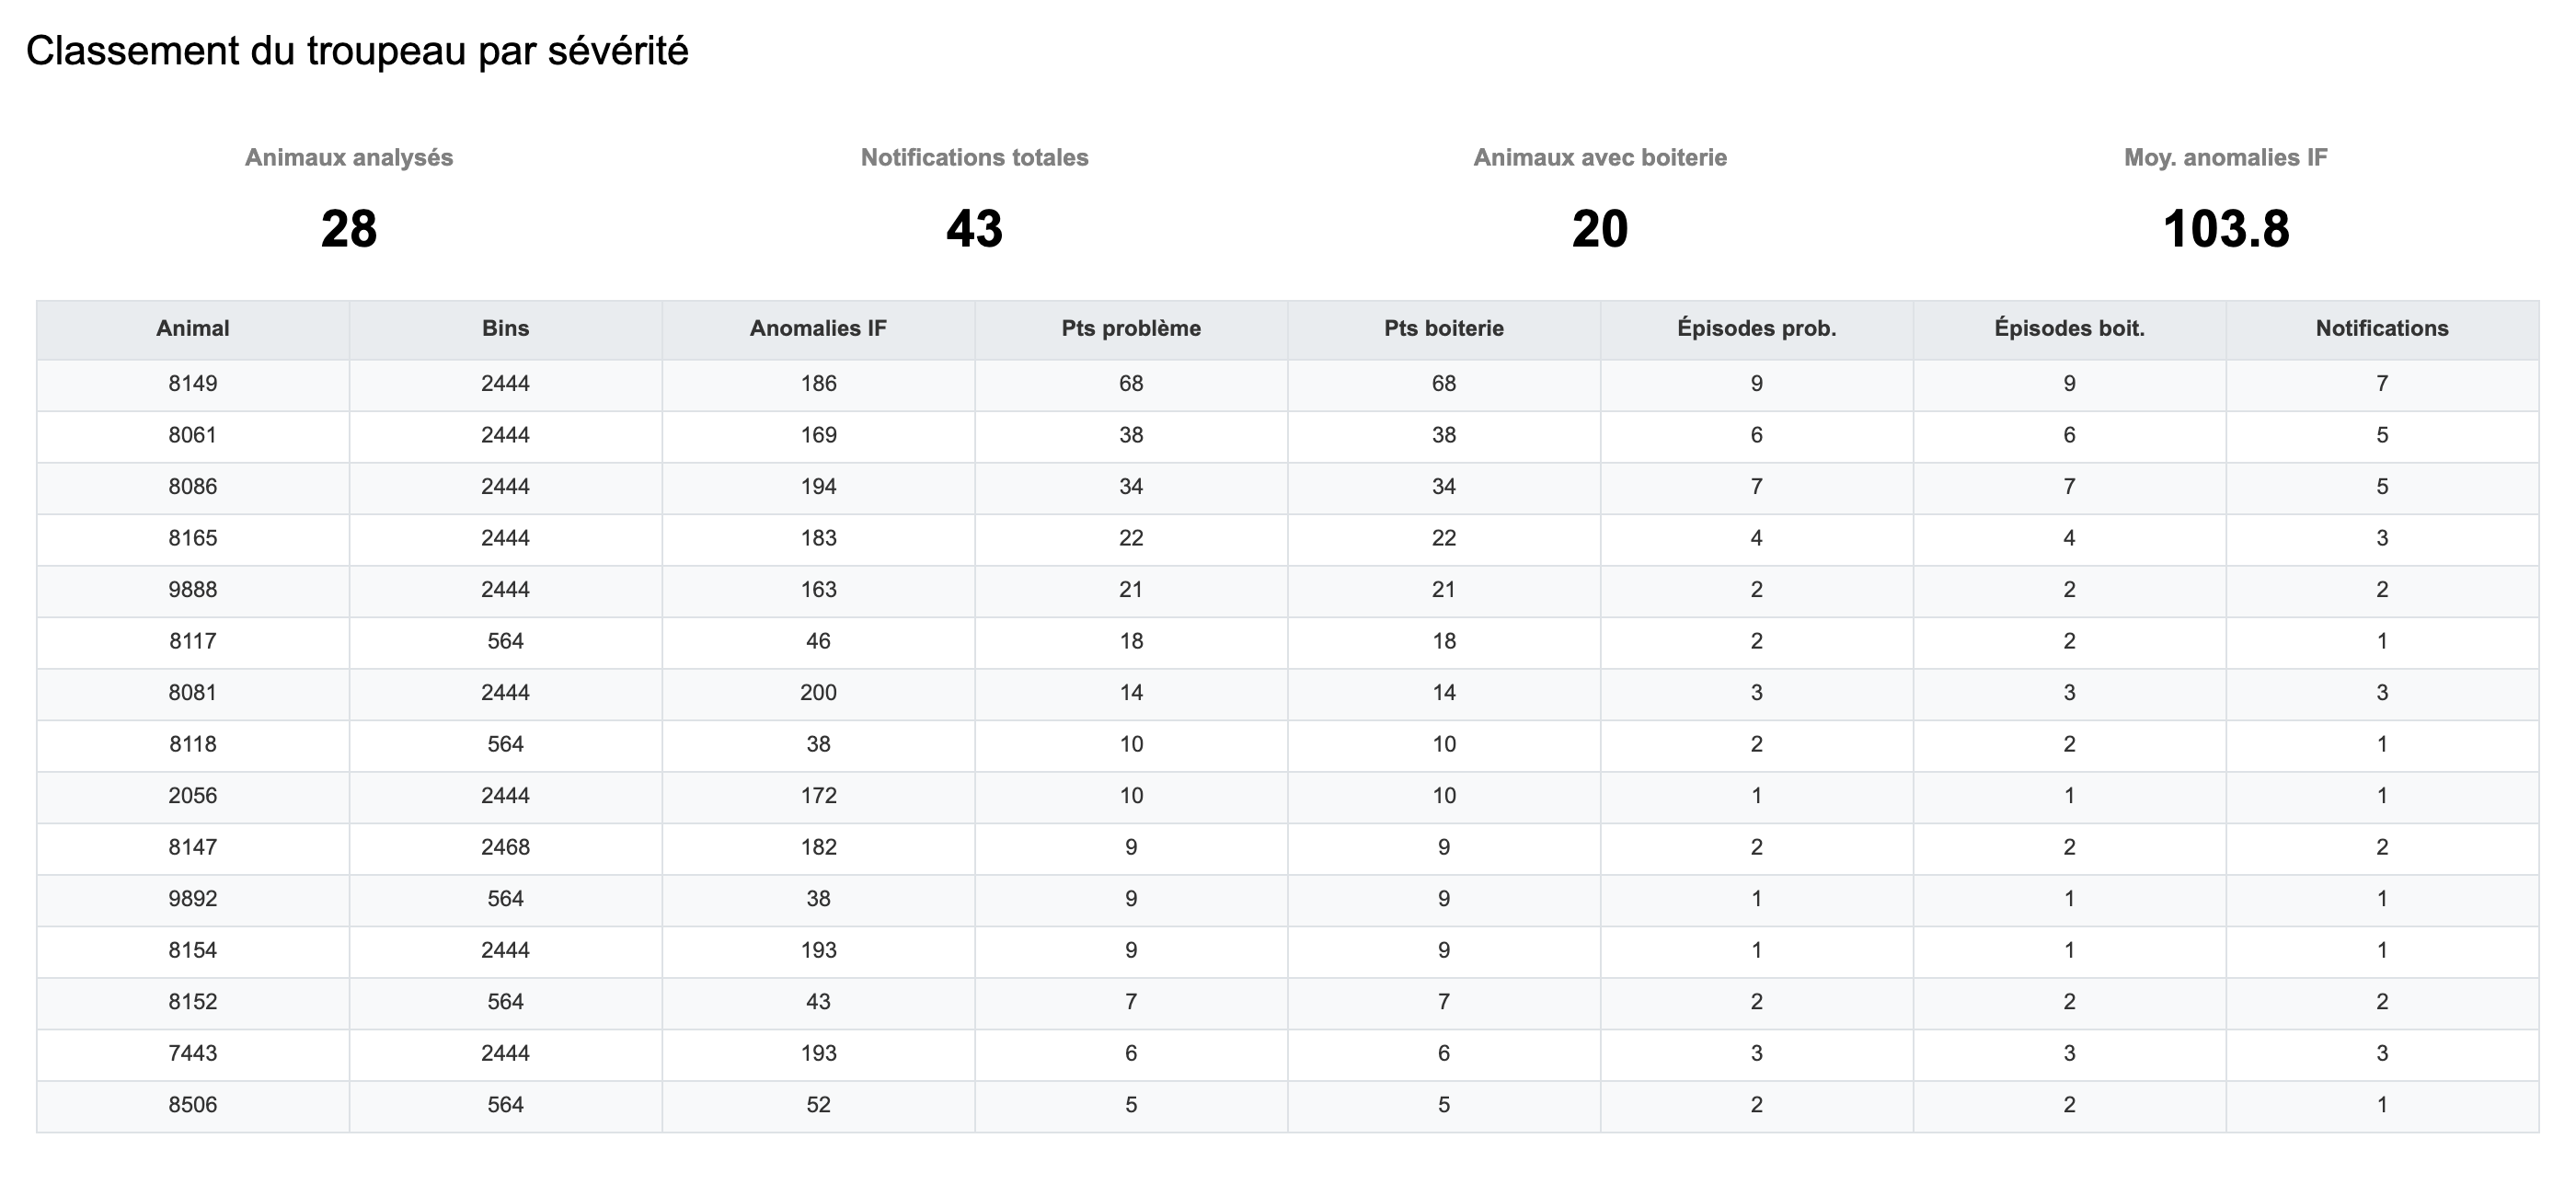
\includegraphics[width=\textwidth]{figures/streamlit_ranking.png}
    \caption{Vue « Classement troupeau » du dashboard.}
    \label{fig:streamlit_ranking}
\end{figure}

\begin{figure}[!htbp]
    \centering
    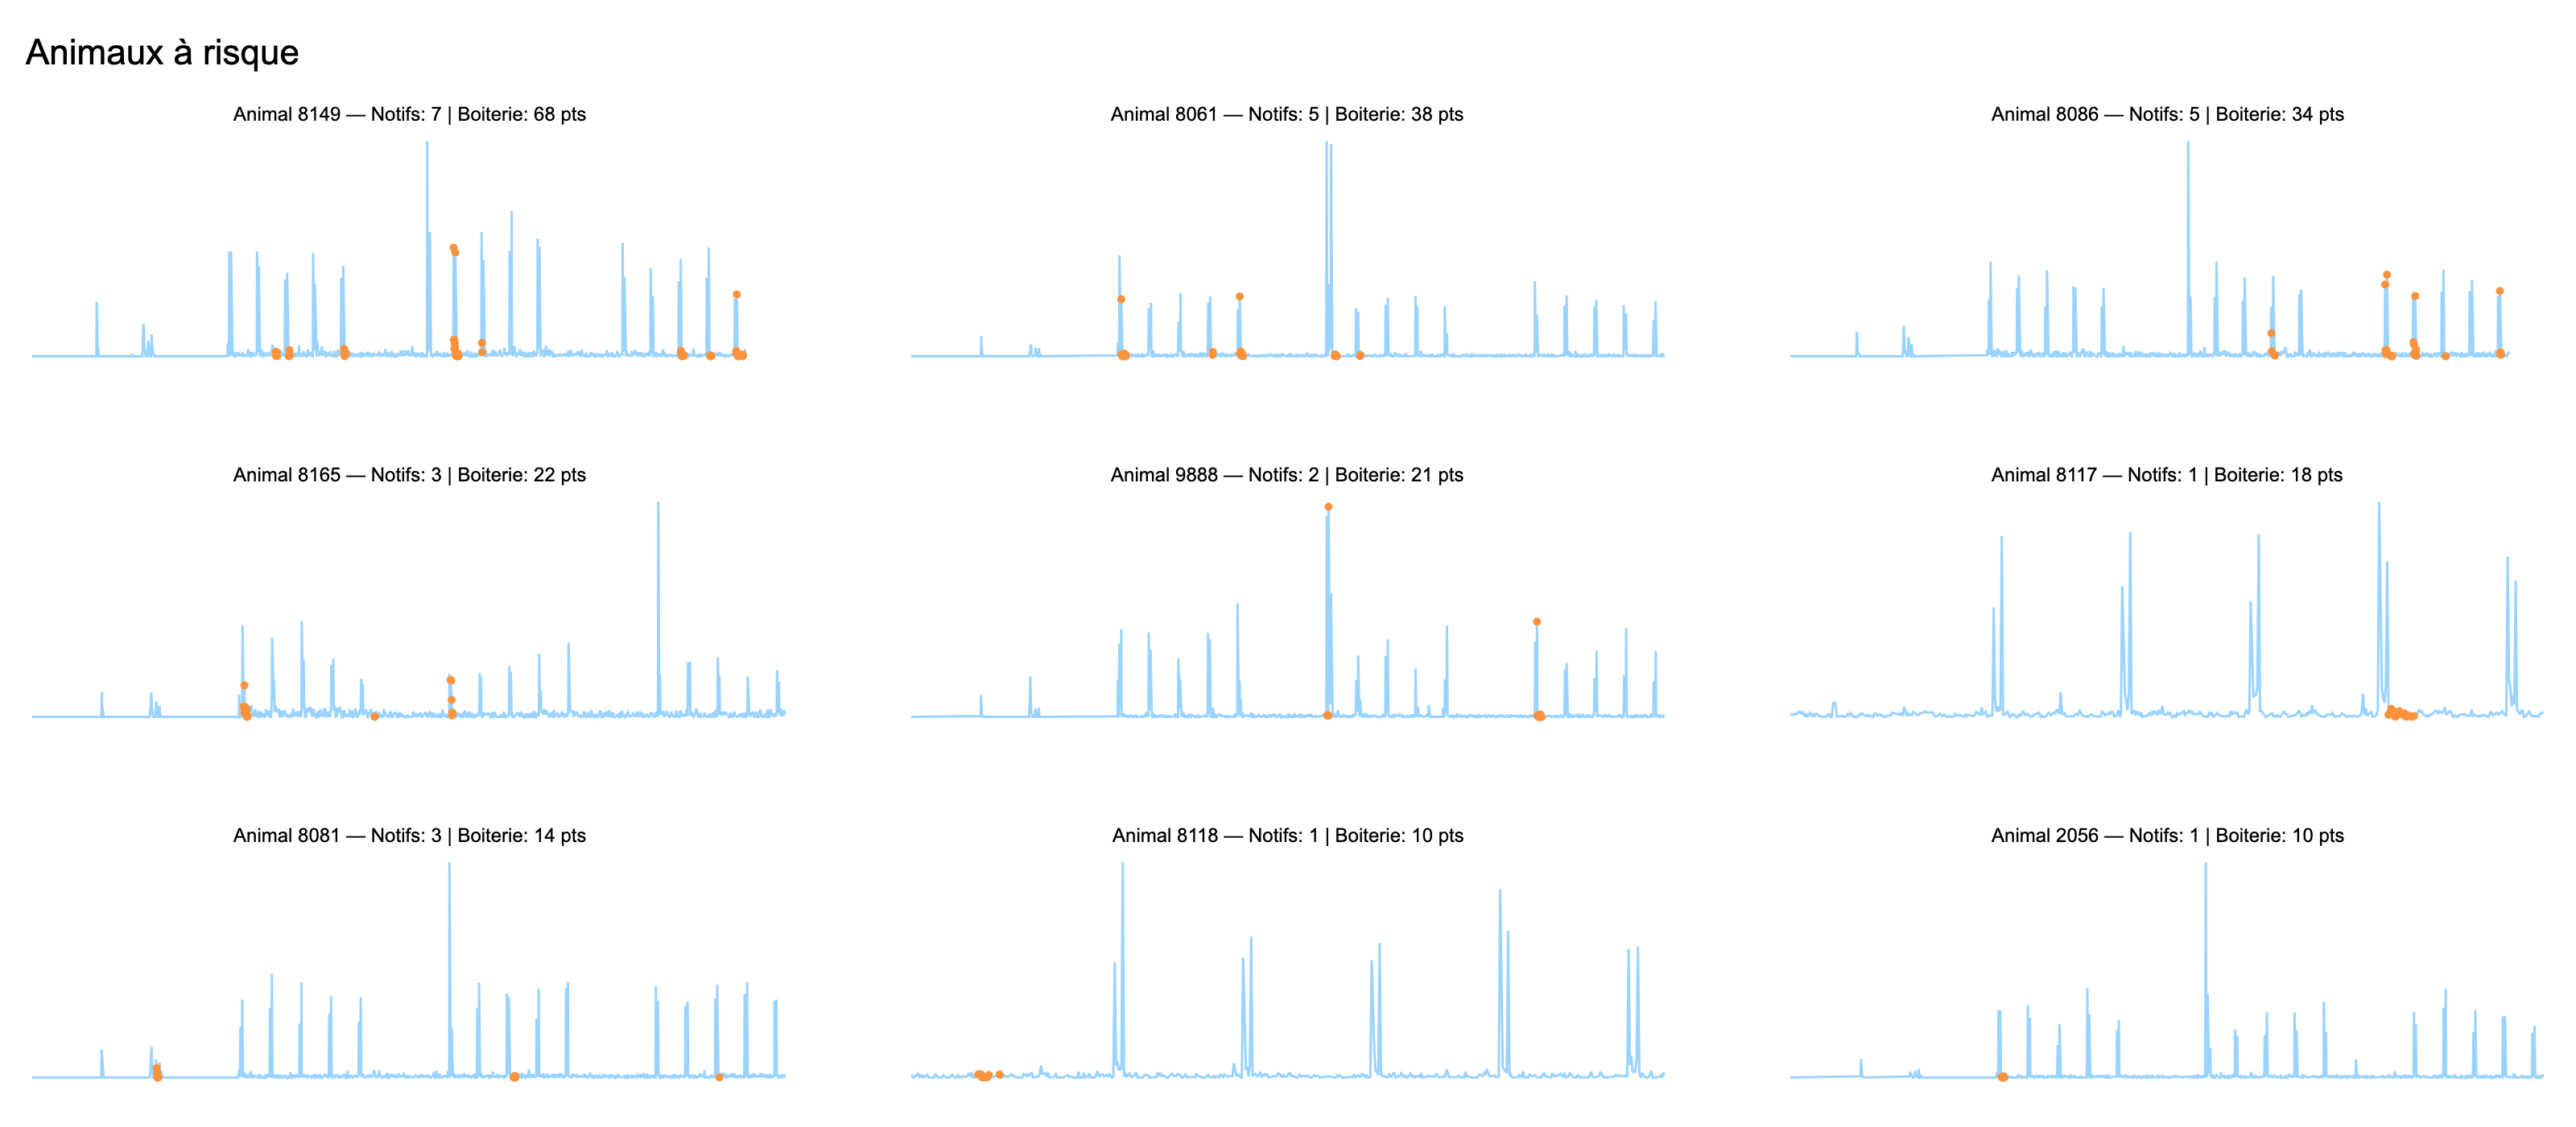
\includegraphics[width=0.92\textwidth]{figures/streamlit_herd.png}
    \caption{Vue « Animaux à risque » du dashboard.}
    \label{fig:streamlit_herd}
\end{figure}

\begin{figure}[!htbp]
    \centering
    
\includegraphics[width=0.75\textwidth]{figures/streamlit_heatmap_compact.png}
    \caption{Carte de chaleur des alertes quotidiennes par animal.}
    \label{fig:streamlit_heatmap}
\end{figure}

\subsection{Score de risque de boiterie (LRS)}
\label{subsec:lrs}

Chaque épisode détecté est accompagné d'un score de risque de boiterie
(\textit{Lameness Risk Score}, LRS), un indicateur continu sur 0--100 quantifiant la
sévérité probable de l'épisode. Contrairement à une décision binaire (alerte / pas
d'alerte), le LRS permet de classer les animaux signalés par ordre de priorité et
d'adapter l'intensité de la réponse terrain.

\textit{Formulation.}
Le LRS est une combinaison pondérée de quatre composantes, chacune normalisée entre 0
et 1 avant agrégation:

\begin{equation}
\text{LRS} = 100 \times \bigl(
    0.30 \cdot c_{\text{multi}} +
    0.30 \cdot c_{\text{persist}} +
    0.20 \cdot c_{\text{mi}} +
    0.20 \cdot c_{\text{if}}
\bigr)
\label{eq:lrs}
\end{equation}

avec:
\begin{itemize}
    \item $c_{\text{multi}}$: taux de cohérence multi-familles dans la fenêtre de
    persistance (fraction des bins où au moins deux familles de signaux présentent
    simultanément une anomalie);
    \item $c_{\text{persist}}$: fraction des bins anormaux dans la fenêtre de
    persistance ($K = 28$~bins, soit 7~h), normalisée par $K$;
    \item $c_{\text{mi}}$: percentile du Motion~Index maximal observé dans la fenêtre
    par rapport à la distribution de la vache, inversé pour la détection de boiterie
    (MI bas = signe de boiterie);
    \item $c_{\text{if}}$: percentile du score IF absolu moyen dans la fenêtre, par
    rapport à la distribution de la vache.
\end{itemize}

\textit{Niveaux d'alerte.}
Le Tableau~\ref{tab:niveaux_alerte} associe des seuils LRS à des niveaux d'alerte et à
un plan d'action clinique tiré des guides de référence
\citep{sprecher1997lameness,ahdb_mobility_scoring_dairy_cows,dairynz_preventing_managing_lameness_guide_2025}.
Les seuils retenus sont indicatifs et calibrés pour la configuration par défaut.

\begin{table}[H]
    \centering
    \small
    \caption{Niveaux d'alerte définis par le Lameness Risk Score (LRS) et plans d'action
    associés.}
    \label{tab:niveaux_alerte}
    \begin{tabular}{cccp{5.5cm}}
        \toprule
        \textbf{Niveau} & \textbf{LRS} & \textbf{Couleur} & \textbf{Plan d'action} \\
        \midrule
        Suspect  & 30--49 & Jaune & Observation au prochain passage (scoring locomoteur) \\
        Probable & 50--74 & Orange & Vérification terrain dans les 24~h; score locomoteur documenté \\
        Critique & 75--100 & Rouge & Examen vétérinaire prioritaire; traitement si score~$\geq$~3 \\
        \bottomrule
    \end{tabular}
\end{table}

\textit{Limites du LRS.}
Le LRS n'est pas calibré comme une probabilité de boiterie au sens clinique: il
reflète l'intensité du signal comportemental, pas la probabilité d'une lésion podiale
confirmée. Les poids de l'Équation~\ref{eq:lrs} sont fixés par jugement expert et non
par optimisation sur des données labellisées. Il est important de noter que le LRS est
un score de classement \textit{post-hoc}: il ne participe pas aux décisions de
détection (épisodes, notifications), qui sont entièrement déterminées par les cinq
paramètres du pipeline (contamination, persistance, seuils MIX, cooldown). Une
variation des poids modifierait l'ordre de priorité des alertes affichées, mais pas
le nombre de détections ni le taux de fausses notifications. La transformation en
niveaux d'alerte constitue donc une aide à la décision opérationnelle, non un
diagnostic. Cette distinction est cohérente avec le positionnement général du système
(voir introduction) et avec les recommandations de la littérature sur
les systèmes de dépistage non diagnostiques \citep{alsaaod2019automatic}.

\subsection{Séparation interface et logique scientifique}

L'interface ne contient aucune logique de détection: elle appelle les mêmes fonctions
que les scripts de validation en ligne de commande. Pour une même configuration et une
même seed aléatoire, l'interface et les scripts produisent des sorties bit à bit
identiques. Les modules d'interface (\texttt{ui/panels\_individual.py},
\texttt{ui/panels\_herd.py}, \texttt{ui/plots.py}) sont isolés dans un répertoire
dédié et ne sont pas importés par le pipeline de détection.

\FloatBarrier
% =====================================================================
\section{Traçabilité}
% =====================================================================

La traçabilité est assurée à trois niveaux complémentaires:

\begin{itemize}
    \item \textit{Versionnage}: l'historique complet des changements de code, de structure
    et de documentation est conservé;
    \item \textit{Intégrité des artefacts}: un manifeste cryptographique (SHA-256) permet de
    vérifier qu'aucun résultat de référence n'a été modifié en place;
    \item \textit{Dépendances figées}: un fichier unique déclare toutes les bibliothèques
    requises et leurs versions, ce qui simplifie la reproduction.
\end{itemize}

Au moment de la présente rédaction, la vérification du manifeste d'intégrité retourne
zéro fichier manquant, zéro fichier modifié et zéro fichier inattendu. Cela confirme
que les validations et benchmarks de référence n'ont pas été altérés par les
réorganisations successives du système.

\subsection{Cycle de vie d'un artefact expérimental}

La Figure~\ref{fig:cycle_artefact} détaille le cycle de vie d'un artefact expérimental,
depuis sa génération jusqu'à sa vérification~: chaque fichier produit par une exécution de
validation est horodaté, haché (SHA-256) et inscrit dans un manifeste, et la
vérification ultérieure compare les hashes actuels au manifeste pour détecter toute
modification. Ce processus, inspiré des pratiques de traçabilité en systèmes d'apprentissage automatique
\citep{sculley2015hidden}, garantit que chaque résultat présenté dans ce mémoire est
rattaché à une configuration précise et à un état du code identifiable.

\begin{figure}[H]
    \centering
    \begin{tikzpicture}[
        stepbox/.style={rectangle, draw=black!60, rounded corners=3pt, minimum height=0.8cm,
                     minimum width=3.5cm, align=center, font=\small, inner sep=10pt},
        arrow/.style={-{Stealth[length=2.5mm]}, thick, black!60},
        check/.style={diamond, draw=rulegreen!70, fill=rulegreen!10, minimum size=0.8cm,
                      font=\scriptsize, inner sep=2pt, aspect=2},
    ]
        \node[stepbox, fill=ifblue!12] (gen) at (0,0) {Génération\\[-7pt](exécution de validation)};
        \node[stepbox, fill=loforange!12] (store) at (5.5,0) {Stockage\\[-7pt](fichier horodaté)};
        \node[stepbox, fill=profgray!10] (hash) at (11,0) {Empreinte\\[-7pt](SHA-256)};

        \node[stepbox, fill=rulegreen!12] (manifest) at (5.5,-2.5) {Inscription\\[-7pt]au manifeste};
        \node[check] (verify) at (11,-2.5) {Vérif.};

        \draw[arrow] (gen) -- node[above, font=\tiny, black!50] {CSV + JSON} (store);
        \draw[arrow] (store) -- node[above, font=\tiny, black!50] {calcul hash} (hash);
        \draw[arrow] (hash) -- (verify);
        \draw[arrow] (store) -- (manifest);
        \draw[arrow] (manifest) -- (verify);

        % Labels résultat
        \node[font=\scriptsize, rulegreen, right=0.3cm of verify] {0 modifié};
    \end{tikzpicture}
    \caption{Cycle de vie d'un artefact expérimental.}
    \label{fig:cycle_artefact}
\end{figure}

Le mécanisme de vérification SHA a permis de détecter deux incidents de modification involontaire lors de
refactorings du code. Dans les deux cas, la vérification SHA a signalé une divergence
avant que les résultats altérés ne soient utilisés dans le mémoire. Les artefacts ont alors
été regénérés à partir de la configuration et du seed d'origine, confirmant la
reproductibilité du pipeline.

Le Tableau~\ref{tab:artefacts_types} résume les types d'artefacts produits par le système
et leur rôle dans la chaîne de traçabilité.

\begin{table}[H]
    \centering
    \caption{Types d'artefacts produits par le pipeline et leur rôle dans la traçabilité.}
    \label{tab:artefacts_types}
    \begin{tabular}{lll}
        \toprule
        \textbf{Type} & \textbf{Format} & \textbf{Contenu} \\
        \midrule
        Résultats de validation & CSV & Métriques par scénario et par seed \\
        Configuration gelée & JSON & Paramètres de l'exécution (seuils, seed, version) \\
        Manifeste d'intégrité & TXT & Hashes SHA-256 de tous les artefacts \\
        Rapport de benchmark & CSV & Temps d'exécution par fraction du corpus \\
        Logs de non-régression & TXT & Résultat des tests automatisés \\
        \bottomrule
    \end{tabular}
\end{table}

\FloatBarrier
% =====================================================================
\section{Reproductibilité et science ouverte}
% =====================================================================

La reproductibilité constitue un enjeu central pour les systèmes d'apprentissage
automatique \citep{pineau2021improving}. Tatman et al. \citep{tatman2018practical}
proposent une taxonomie pratique distinguant trois niveaux de reproductibilité dans la
recherche en apprentissage automatique~: la reproductibilité des résultats, la reproductibilité de l'analyse
et la reproductibilité des données. Le présent pipeline vise les trois niveaux.
Plusieurs mesures ont été adoptées pour garantir la transparence des résultats,
en cohérence avec les principes FAIR \citep{wilkinson2016fair}.

L'environnement d'exécution est minimaliste: Python~3.10+, scikit-learn~1.x, pandas~2.x
et NumPy, sans GPU ni matériel dédié. L'ensemble des dépendances est déclaré dans un
fichier unique (\texttt{requirements.txt}). Le pipeline s'exécute en environ
0.6~seconde par vache sur un ordinateur standard, ce qui rend la reproduction accessible
sans infrastructure spécialisée. Toutes les opérations stochastiques utilisent un seed
explicite, garantissant la reproductibilité bit-à-bit sur une version donnée des
dépendances.

Les 9\,504~exécutions de validation sont stockés en formats ouverts (CSV, JSON) et
protégés par un manifeste d'intégrité SHA-256 couvrant 1\,340~fichiers d'artefacts. Ce
manifeste vérifie systématiquement l'absence de fichiers manquants, modifiés ou
inattendus. Au moment de la rédaction, la vérification retourne zéro anomalie sur
l'ensemble des artefacts. Le versionnage Git et les tests de non-régression
(Tableau~\ref{tab:tests_strategie}) garantissent que les réorganisations du code ne
modifient pas les résultats scientifiques.

Les protocoles expérimentaux sont documentés par une combinaison de notebooks Jupyter et
de scripts versionnés avec le projet: validations manuelles (v2, v2.1), validations
robustes (v4, v5.1, v5.2) et comparaison exploratoire IF/LOF. Ces artefacts constituent
à la fois un protocole expérimental explicite et une preuve d'exécution sur le corpus
étudié.

Le code source du pipeline, les scripts de validation et les paramètres gelés sont
versionnés dans un dépôt Git privé. La version de référence du mémoire correspond au
tag \texttt{memoire-v2} et est décrite dans le manifeste
\path{data/memoire_archive_manifest_v2.json} ; le code et les artefacts non
confidentiels sont disponibles sur demande auprès de l'auteur. Les données brutes
capteurs ne peuvent pas être diffusées pour des raisons de confidentialité, mais les
profils d'injection, les paramètres de validation, les manifestes SHA-256 et les artefacts
synthétiques documentés en Annexe~\ref{annexe:validation} permettent de reproduire la
démarche expérimentale sur de nouvelles données.

\vspace{0.5em}
\noindent
L'architecture étant définie et les mécanismes de reproductibilité en place, le chapitre
suivant présente les résultats expérimentaux obtenus lors des campagnes de validation. On y
évalue le pipeline sur 9\,504~exécutions, en mesurant la détection, la précision
temporelle, les fausses alertes et la stabilité inter-campagnes.
